% This is "sig-alternate.tex" V2.1 April 2013
% This file should be compiled with V2.5 of "sig-alternate.cls" May 2012
%
% This example file demonstrates the use of the 'sig-alternate.cls'
% V2.5 LaTeX2e document class file. It is for those submitting
% articles to ACM Conference Proceedings WHO DO NOT WISH TO
% STRICTLY ADHERE TO THE SIGS (PUBS-BOARD-ENDORSED) STYLE.
% The 'sig-alternate.cls' file will produce a similar-looking,
% albeit, 'tighter' paper resulting in, invariably, fewer pages.
%
% ----------------------------------------------------------------------------------------------------------------
% This .tex file (and associated .cls V2.5) produces:
%       1) The Permission Statement
%       2) The Conference (location) Info information
%       3) The Copyright Line with ACM data
%       4) NO page numbers
%
% as against the acm_proc_article-sp.cls file which
% DOES NOT produce 1) thru' 3) above.
%
% Using 'sig-alternate.cls' you have control, however, from within
% the source .tex file, over both the CopyrightYear
% (defaulted to 200X) and the ACM Copyright Data
% (defaulted to X-XXXXX-XX-X/XX/XX).
% e.g.
% \CopyrightYear{2007} will cause 2007 to appear in the copyright line.
% \crdata{0-12345-67-8/90/12} will cause 0-12345-67-8/90/12 to appear in the copyright line.
%
% ---------------------------------------------------------------------------------------------------------------
% This .tex source is an example which *does* use
% the .bib file (from which the .bbl file % is produced).
% REMEMBER HOWEVER: After having produced the .bbl file,
% and prior to final submission, you *NEED* to 'insert'
% your .bbl file into your source .tex file so as to provide
% ONE 'self-contained' source file.
%
% ================= IF YOU HAVE QUESTIONS =======================
% Questions regarding the SIGS styles, SIGS policies and
% procedures, Conferences etc. should be sent to
% Adrienne Griscti (griscti@acm.org)
%
% Technical questions _only_ to
% Gerald Murray (murray@hq.acm.org)
% ===============================================================
%
% For tracking purposes - this is V2.0 - May 2012

\documentclass{sig-alternate}

\usepackage{listings}
\usepackage{color}

\newcommand\TODO[1]{{[\color{red}#1]}}

\begin{document}

\CopyrightYear{2017} 
\setcopyright{acmlicensed}
\conferenceinfo{SIGCSE '17,}{March 08 - 11, 2017, Seattle, WA, USA}
\isbn{978-1-4503-4698-6/17/03}\acmPrice{\$15.00}
\doi{http://dx.doi.org/10.1145/3017680.3017708}

% --- End of Author Metadata ---

\title{Computing with CORGIS:\\ Diverse, Real-world Datasets for Introductory Computing}
%
% You need the command \numberofauthors to handle the 'placement
% and alignment' of the authors beneath the title.
%
% For aesthetic reasons, we recommend 'three authors at a time'
% i.e. three 'name/affiliation blocks' be placed beneath the title.
%
% NOTE: You are NOT restricted in how many 'rows' of
% "name/affiliations" may appear. We just ask that you restrict
% the number of 'columns' to three.
%
% Because of the available 'opening page real-estate'
% we ask you to refrain from putting more than six authors
% (two rows with three columns) beneath the article title.
% More than six makes the first-page appear very cluttered indeed.
%
% Use the \alignauthor commands to handle the names
% and affiliations for an 'aesthetic maximum' of six authors.
% Add names, affiliations, addresses for
% the seventh etc. author(s) as the argument for the
% \additionalauthors command.
% These 'additional authors' will be output/set for you
% without further effort on your part as the last section in
% the body of your article BEFORE References or any Appendices.

\numberofauthors{1} %  in this sample file, there are a *total*
% of EIGHT authors. SIX appear on the 'first-page' (for formatting
% reasons) and the remaining two appear in the \additionalauthors section.
%
 \author{
 \alignauthor
 Austin Cory Bart, Ryan Whitcomb, Dennis Kafura, Clifford A. Shaffer, and Eli Tilevich\\
 \smallskip
        \email{\{acbart, rwhit94, kafura, shaffer, tilevich\}@vt.edu}\\
        \smallskip
 	   \affaddr{Department of Computer Science, Virginia Tech,}
 	   \affaddr{Blacksburg, VA 24061, USA}
 }

\date{26 August 2016}
% Just remember to make sure that the TOTAL number of authors
% is the number that will appear on the first page PLUS the
% number that will appear in the \additionalauthors section.

\maketitle
\begin{abstract}

To successfully bring introductory computing to non-CS majors, one needs to create a curriculum that will appeal to students from diverse disciplines.
Several educational theories emphasize the need for introductory contexts that align with students' long-term goals and are perceived as useful.
Data Science, using algorithms to manipulate real-world data and interpreting the results, has emerged as a field with cross-disciplinary value, and has strong potential as an appealing context for introductory computing courses.
However, it is not easy to find, clean, and integrate datasets that will satisfy a broad variety of learners.
The CORGIS project (\url{https://think.cs.vt.edu/corgis}) enables instructors to easily incorporate data science into their classroom.
Specifically, it provides over 40 datasets in areas including history, politics, medicine, and education.
Additionally, the CORGIS infrastructure supports the integration of new datasets with simple libraries for Java, Python, and Racket, thus empowering introductory students to write programs that manipulate real data.
Finally, the CORGIS web-based tools allow learners to visualize and explore datasets without programming, enabling data science lessons on day one.
We have incorporated CORGIS assignments into an introductory course for non-majors to study their impact on learners' motivation, with positive initial results.
These results indicate that external adopters are likely to find the CORGIS tools and materials useful in their own pedagogical pursuits.
\end{abstract}


% The code below should be generated by the tool at
% http://dl.acm.org/ccs.cfm
% Please copy and paste the code instead of the example below. 

\begin{CCSXML}
<ccs2012>
<concept>
<concept_id>10002951.10002952.10003219</concept_id>
<concept_desc>Information systems~Information integration</concept_desc>
<concept_significance>500</concept_significance>
</concept>
<concept>
<concept_id>10002951.10002952</concept_id>
<concept_desc>Information systems~Data management systems</concept_desc>
<concept_significance>100</concept_significance>
</concept>
<concept>
<concept_id>10003456.10003457.10003527.10003528</concept_id>
<concept_desc>Social and professional topics~Computational thinking</concept_desc>
<concept_significance>300</concept_significance>
</concept>
<concept>
<concept_id>10003456.10003457.10003527.10003530</concept_id>
<concept_desc>Social and professional topics~Model curricula</concept_desc>
<concept_significance>300</concept_significance>
</concept>
<concept>
<concept_id>10003456.10003457.10003527.10003539</concept_id>
<concept_desc>Social and professional topics~Computing literacy</concept_desc>
<concept_significance>100</concept_significance>
</concept>
</ccs2012>
\end{CCSXML}

\ccsdesc[500]{Information systems~Information integration}
\ccsdesc[100]{Information systems~Data management systems}
\ccsdesc[300]{Social and professional topics~Computational thinking}
\ccsdesc[300]{Social and professional topics~Model curricula}
\ccsdesc[100]{Social and professional topics~Computing literacy}



%
% End generated code
%

%
%  Use this command to print the description
%
\printccsdesc

\keywords{data science; pedagogy; motivation; authenticity; real-world data; big data; corgis; Computational thinking}

\newpage
\section{Introduction}

As computing skills become required for an increasing number of disciplines, CS educators are meeting the demand by creating courses for non-CS majors.
Students are drawn from many disciplines, including the sciences, arts, and humanities, and they have myriad, divergent career paths before them distinct from those of Computer Science majors.
This different population needs a different approach, one that all students will perceive as authentic and beneficial, while simultaneously enabling problems of a computational nature~\cite{guzdial2006imagineering}.

We suggest that most students would benefit from computational techniques that empower them to manage the ever-growing amounts of data present in every field~\cite{manyika2011big}.
Therefore, a Data Science context, where students write algorithms to manipulate real-world data and interpret the results, could provide a compelling context.
However, integrating data into introductory courses creates challenges for instructors, both pedagogically and technologically.
Finding many, varied datasets can be difficult, and they often require cleaning to be suitable for beginners (e.g., to remove missing values, to scale it to the appropriate size, to choose a convenient format).
To overcome these problems, we present here the open-source CORGIS project, the \textbf{C}ollection \textbf{O}f \textbf{R}eally \textbf{G}reat and \textbf{I}nteresting data\textbf{S}ets, which makes a wide variety of student-ready datasets available.
Our materials are free and open-source, available at  \texttt{\url{https://think.cs.vt.edu/corgis}}.

This paper begins with a brief review of relevant educational theory and existing projects in this space.
We then briefly describe the technical innovations of the CORGIS project and its pedagogical affordances, and specific ways that it can be used in a course.
We report and evaluate results of an intervention conducted using the software.
Finally, we discuss the future of the project.


\section{Educational Theory}

Educational Theory grounds the development of the CORGIS project.
We use Situated Learning Theory~\cite{lave-situated} to better understand how students learn, and the MUSIC Model of Academic Motivation~\cite{jones-description} to better understand why students choose to engage.

Situated Learning Theory suggests that authentic contexts are crucial for learners.
Originally proposed by Lave and Wenger, SL Theory argues that tasks in the learning environment should parallel real-world tasks, in order to maximize the authenticity of the experience~\cite{lave-situated}.
Some interpretations of this theory draw a distinction between the content (e.g., learning to program) and the context (e.g., by creating a video game), and stress that proper contextualization is important for students' comprehension and investment~\cite{situated-cognition}.

In our research, we rely on the MUSIC Model of Academic Motivation~\cite{jones-description}.
Built as a meta-model, it incorporates many existing theories and is tailored particularly for education.
The model distinguishes between students' situational \textit{interest} in an academic activity and their sense of the \textit{usefulness} of the activity to their long-term career goals.
We connect this distinction to the different contexts available to introductory courses.
Creating games and animations, for example, appeals to students' situational interest, while we posit that data science will appeal more to students' sense of usefulness.
The MUSIC model also incorporates students' expectation for appropriate \textit{Successes} when learning, their sense of \textit{eMpowerment} within the activity, and their perception of their instructors \textit{Caring} towards them.

From these two theories, we hypothesize that Data Science will be a beneficial context for students, since students will perceive the context as closely related to their career goals.

\section{Related and Prior Work}

The use of data analysis for contextualization represents an actively growing movement~\cite{Anderson, Sullivan:2013,Hall-Holt:2015,DePasquale:2006}.
Upper division courses have employed situated learning experiences using data of varying size and complexity for several years~\cite{Egger,datamining}.
However, this prior work has little evaluation of the impacts of data science in introductory education~\cite{Sullivan:2013,DePasquale:2006}.

The RealTimeWeb project (RTW)~\cite{realtimeweb} made it easy for instructors to bring web-based, rapidly-updating data into their introductory classrooms by writing light-weight specifications of remote data streams.
CORGIS is similar to RTW, moving from a small collection of web-based data to a wide collection of local data.
The change was motivated by the authors perceived scarcity of quality, real-time datasets.
And, while the technical challenges of integrating real-time data are interesting, they are of secondary importance to the value of having a diversity of relevant datasets.

The BigDataCSE project of Hamid~\cite{Hamid2016} takes real-time data access in a different direction by reducing the technical requirements on instructors even further.
The library uses sophisticated reflection techniques to automatically infer the structure of data, so that students can access any desired URL endpoint and receive structured data.
Although it provides a flexible architecture, this project does not attempt to provide datasets, making it more appropriate for advanced students who can find their own data to work with.

The BRIDGES project provides students with visualizations of their algorithms on datasets~\cite{burlinson2016bridges}.
BRIDGES does not focus on organizing datasets directly, but incorporates existing datasets (including some directly from the CORGIS project).
The use of visualizations can help students understand the interaction between their algorithms and data.

\begin{figure}[!ht]
    \centering
    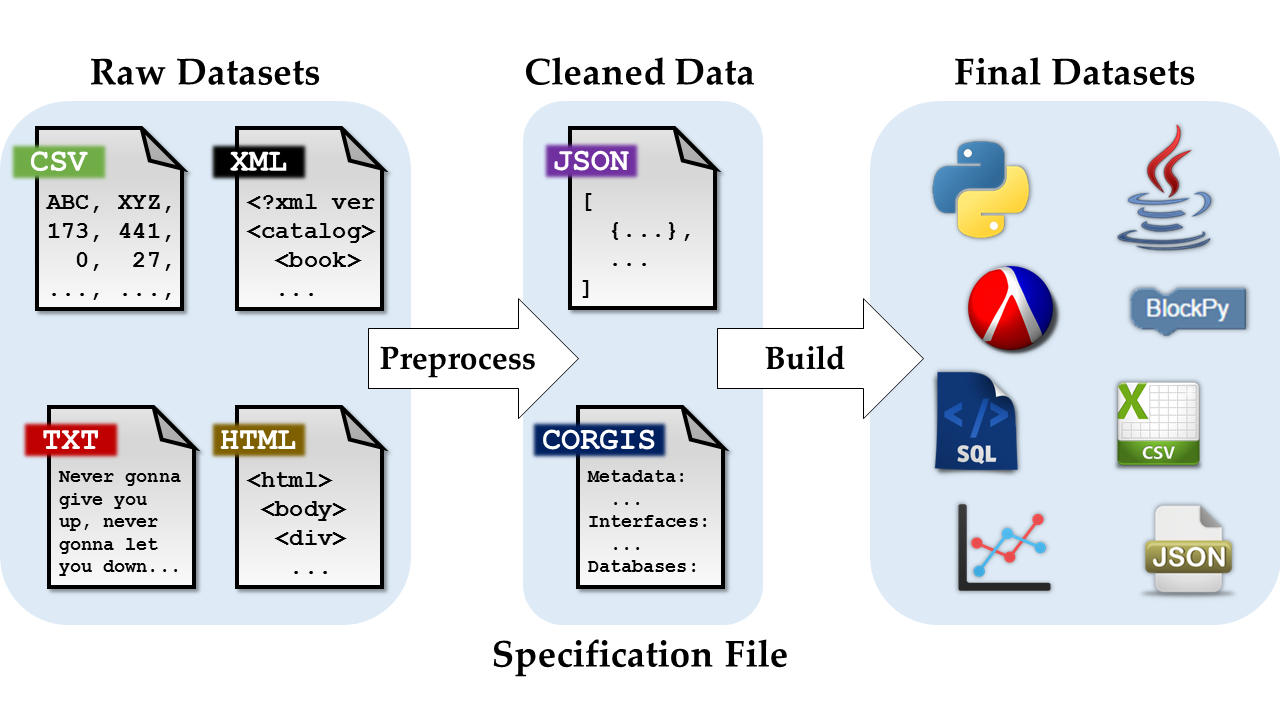
\includegraphics[width=.47\textwidth]{graphics/process}
    \vspace{-\bigskipamount}
    \vspace{-\smallskipamount}
    \caption{How datasets are added to CORGIS}
    \label{fig:corgis-build}
\end{figure}


\section{Design}

The CORGIS project aspires to have multiple (3-4) data\-sets relevant to each major career path that potential students might seek.
To achieve this, we draw on data from wide-ranging, open-access sources including governments, research publications, journalists, non-profits, and industry.
Figure~\ref{fig:corgis-build} provides an overview of how datasets are added to the CORGIS project. 

First, real-world data is collected and preprocessed into a ``clean'' state.
Most of the human effort for the project comes at this phase, as organizing a dataset requires expertise.
Figure~\ref{fig:classics-data-map} shows a representation for the cleaned structure of a dataset.
Every dataset becomes a list of hierarchical maps (a tree), where the leaf nodes are simple data types: numbers, text, and booleans.

Next, high-level specification files are written to describe the metadata, fields, and interfaces for a cleaned dataset.
All CORGIS datasets have interfaces that can be used to slice the data.
The weather dataset, for example, provides ``Get Temperature'' and ``Get Past Temperatures'' that return an integer and a list of integers, respectively.
These specification files can be validated by the system using a custom compiler.

The CORGIS infrastructure uses the specification file and associated dataset to automatically generate a number of student-ready materials.

\textbf{Language Libraries: } The CORGIS project currently supports the generation of Python, Java, and Racket libraries.
Figure \ref{fig:example-usage} gives examples of how a generated library can be used in these languages.
Code and supporting documentation for a library are generated by filling out templates using the Jinja2 templating library.
Interfaces from the specification file generate functions that execute queries.
A SQLite database is also generated to store the data, rather than the original JSON file, for performance reasons.

\begin{figure}[hb!]
\begin{lstlisting}[language=Python,basicstyle=\scriptsize]
# Python
import crime
crimes = crime.get_all()
\end{lstlisting}
\begin{lstlisting}[language=Lisp,basicstyle=\scriptsize]
; Racket
(require crime)
(define reports (crime-get-all))
\end{lstlisting}
\begin{lstlisting}[language=Java,basicstyle=\scriptsize]
// Java
import corgis.crime.StateCrimeLibrary;
import corgis.crime.domain.Report;

public class Main {
  public static void main(String[] args) {
    StateCrimeLibrary stateCrimeLibrary = 
         new StateCrimeLibrary();
    ArrayList<Report> reports = 
         stateCrimeLibrary.getAllCrimes();
  }
}
\end{lstlisting}
\vspace{-\medskipamount}
\caption{Example of using a CORGIS library}
\label{fig:example-usage}
\end{figure}

\begin{figure}[ht!]
    \centering
    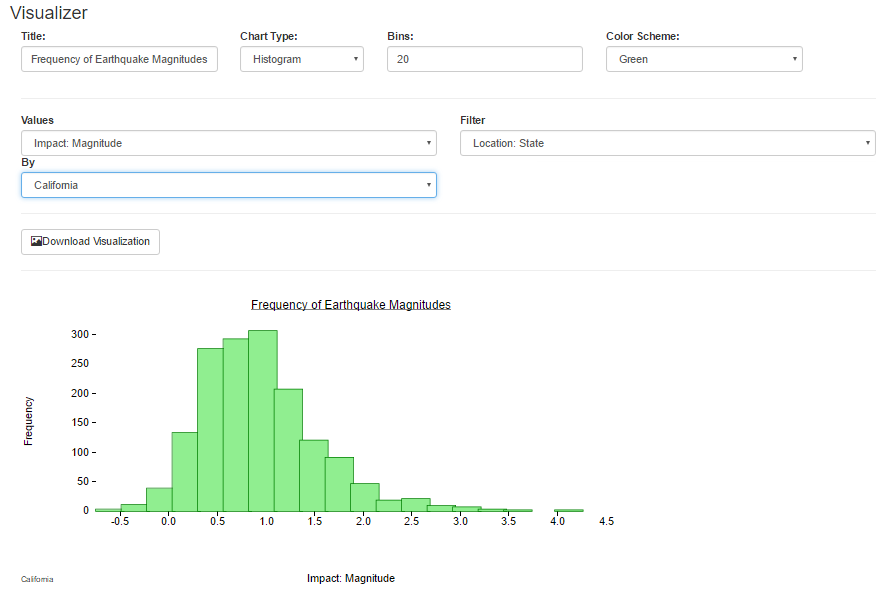
\includegraphics[width=.47\textwidth]{graphics/visualizer}
    \vspace{-\smallskipamount}
    \caption{The CORGIS visualizer}
    \label{fig:visualizer}
    \vspace{-\medskipamount}
\end{figure}

\newpage
\textbf{Visualizer} The Visualizer allows students to engage with datasets in their browser without programming, as shown in Figure~\ref{fig:visualizer}.
Users can generate histograms, line plots, scatter plots, and bar charts for any supported dataset.
Bar charts are categorized by the indexes from the specification file.
Datasets can also be filtered on indexed fields when generating charts.
Although not as powerful as a full programming environment, the Visualizer empowers students to work with real-world data without specialized training.


\textbf{Explorer} Separate from data content, students can explore the structure of a dataset using the Explorer.
The hierarchy of data is explored through chained windows.
Clicking a field in a map, for instance, might open a new map's window, which in turn might have atomic fields or links to further maps.


\textbf{Raw Data Files} Language bindings simplify access to datasets, but some instructors may want students to use more traditional methods.
Therefore, we expose datasets in popular raw formats: JSON, SQL, and CSV.
The SQL database represents each child map as a distinct table, linked with a primary key.
The CSV table is a flattened representation of the data, using the key hierarchy to disambiguate column names.

\textbf{The CORGIS Gallery} Language bindings, data files, and the Visualizer are all accessible through a user-friendly Gallery, shown in Figure~\ref{fig:corgis-gallery}.
Every dataset is documented with a list of content tags to help students search for a relevant dataset.

\begin{figure}[hb!]
    \centering
    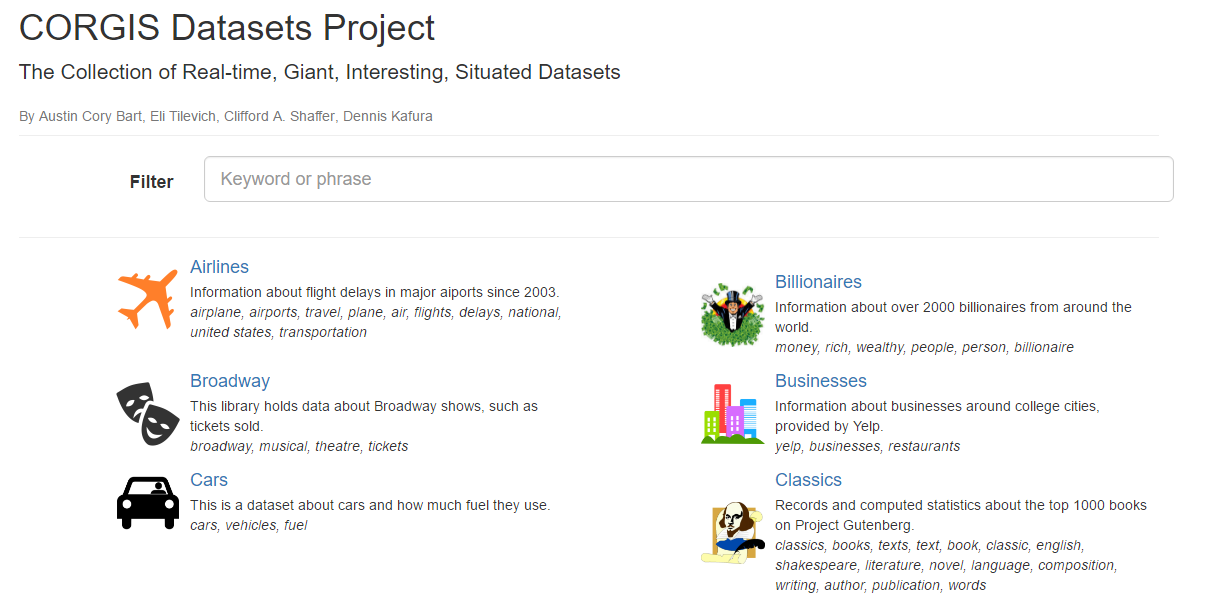
\includegraphics[width=.47\textwidth]{graphics/gallery}
    \caption{The CORGIS gallery}
    \label{fig:corgis-gallery}
\end{figure}


\newpage
\section{Assignments}

CORGIS can be integrated into introductory courses in a number of ways.
In this section, we describe how we have used the tools in an existing course on Computational Thinking for non-majors.
This course teaches basic programming in a Data Science context.
Much of the CORGIS development has been driven by the needs of the course.

The major motivational goal of integrating CORGIS is to align assignments with students' career goals.
However, assignments also benefit from the wide variety of the CORGIS collection.
Learners can choose their own datasets to explore things related to their own interests and career goals, increasing their sense of agency.

%\subsection{Abstraction}

%Students must understand the relationship between the process of \textit{abstracting} and \textit{interpreting} data.
%In the context of this project, we describe Abstraction as the process of simplifying and representing real-world phenomenon using concrete, computable properties.
%The process of abstraction necessarily throws away context and data that is not practical for solving problems of an expected stakeholder.


\subsection{Exploratory Analysis}

The Visualizer facilitates early exploration of datasets, without the need to program.
In the beginning of our course, students generate graphs in groups (each group is assigned a dataset) and then on their own (free to choose their own dataset).
They are tasked with creating visualizations to explore questions about the distribution, trends, and relationships of the data.
For example, in the crime dataset, they can identify the downward trend of violent crime rates over time in different states.
This is an opportunity to discuss how complex, real-world entities and phenomenon can be represented with computable abstractions (e.g., numbers).
Additionally, this gives students practice with selecting and interpreting different kinds of charts. 
In our experience, many students struggle with aspects of graphs such as distinguishing bar charts and histograms, or knowing when to use line plots.

\subsection{Practice Problems}

When students start programming, we give them practice problems contextualized with CORGIS datasets.
Although the scope of these problems is similar to those found in systems like CodingBat~\cite{parlante2015codingbat}, the problems can be more realistic.
The complexity of using complete datasets is avoided by using the simpler interfaces exposed for libraries.
For example, students might be tasked with writing a program to print whether an umbrella is necessary depending on the weather in their current city (requiring only a function call to the Weather library, an if-statement, and the print statement).
A wide range of programming topics can be contextualized with the CORGIS libraries, including collection-based iteration, decisions, printing and visualization, and functions.
In our course, datasets are incorporated through a block-based programming environment~\cite{bart-blockpy} and then in a regular Python programming environment, but the libraries and raw datasets could be used in a variety of development environments.

\subsection{Data Mapping}

A learning goal in our course is for students to be able to navigate and manipulate complex data structures (e.g., nested lists and dictionaries).
We direct students to create a hand-written ``data map'', like the one in Figure~\ref{fig:classics-data-map}.
This diagram visually describes the structure of the dataset, and students use it as a guide to developing the necessary code constructs (e.g., iteration, dictionary access), much as they would navigate a real map to find a path in a maze.
Because of the vastness of most datasets' structure, students must be judicious in what branches and leaves of the structure they diagram, in anticipation of what they will use in their code.

\begin{figure}[ht!]
    \centering
    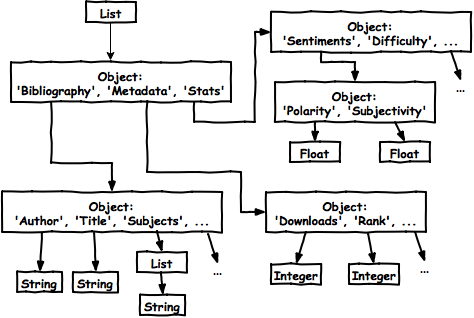
\includegraphics[width=.47\textwidth]{graphics/classics-data-map}
    \caption{Partial data map for the Classics library}
    \label{fig:classics-data-map}
\end{figure}


\subsection{Large-scale Data Analysis}

For our course's final project, students are tasked with formulating questions about a  dataset of their own choosing, writing code to create visualizations, and then interpreting those visualizations using relevant domain knowledge.
We claim that this is an authentic form of assessment for students in the course, modeling what they might do if they were to incorporate data science into their own careers to solve open-ended problems using computational techniques.
The nature of the CORGIS data structure requires them to use a number of coding constructs, including iteration and dictionary access.
In addition to their code, students must turn in a 5-minute video presentation reporting their results.
Students share their videos with each other to demonstrate the breadth available in computing.
Students are required to describe the abstractions used in the project and the inherent limitations of the dataset.
This turns a weakness in the dataset into an important learning experience for the students.
The final project is assessed both by course staff and peers.


\section{Evaluation}

In this section, we evaluate the CORGIS project's progress in two ways.
First, we present empirical metrics for the datasets.
Second, we present survey results from a course that incorporated real-world data through CORGIS.

\subsection{Metrics}
\label{sec:structure-metrics}

At the time of writing, there are over 40 datasets in the CORGIS gallery, and we are actively working to add more datasets.
The left graph of Figure~\ref{fig:metrics} reveals characteristics of the datasets within the corpus.
If the data's structure is seen as a tree, the Average Branch Factor (ABF) is the mean number of fields in a child.
The height of a dataset is the maximal depth of the tree, and Fields is the number of leaves.
Rows is the number of records in the dataset, while size is the amount of disk space used by a dataset.
Although we are pleased with the narrow distribution on some of the attributes (e.g., heights), the dispersion of ABF and Fields suggests that some datasets need to have fewer fields organized into more branches.


\begin{figure}[ht!]
    \centering
    \begin{minipage}[b]{0.225\textwidth}
    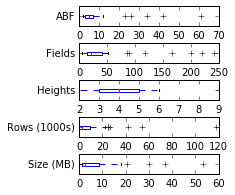
\includegraphics[width=\textwidth]{graphics/characteristics-graph}
    \end{minipage}
    \hfill
    \begin{minipage}[b]{0.225\textwidth}
    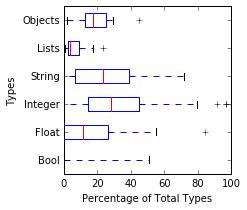
\includegraphics[width=\textwidth]{graphics/type-percentages}
    \end{minipage}
    \caption{Distribution of structure, characteristics, and types across all datasets}
    \label{fig:metrics}
\end{figure}

The right graph of Figure~\ref{fig:metrics} shows the distribution of atomic and composite types within datasets.
Numeric and string types dominate.
Most datasets have few or no boolean types, and few datasets have more than just the top-level list (which is present in every dataset).
The x-axis shows percentages of all types within the dataset, with numerics and strings as the most common.
The chart does not distinguish between different types of string values, such as unique identifiers, URLs, classification codes, or textual data.

\begin{figure}[ht!]
    \centering
    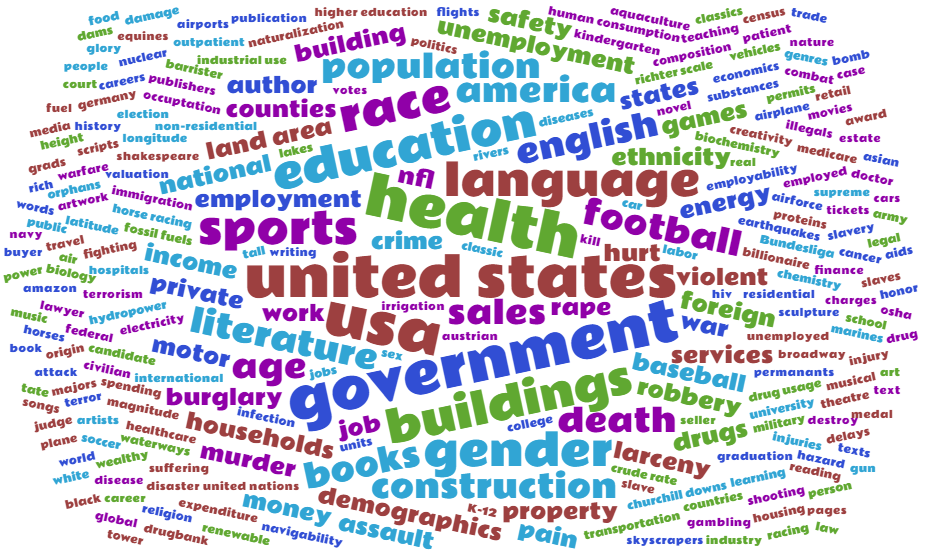
\includegraphics[width=.47\textwidth]{graphics/corgis-cloud-color}
    \caption{CORGIS datasets word cloud of tags}
    \label{fig:corgis-cloud}
\end{figure}

Figure~\ref{fig:corgis-cloud} shows a word cloud of all the descriptive tags associated with the CORGIS datasets.
This graphic illustrates the range of datasets associated with the project.
This also reveals certain biases and trends in the selection of datasets.
United States, for instance, is the single largest word in the cloud.
Unfortunately, this graphic is not helpful in finding under-represented career paths and disciplines, which is a key problem for the project.

\subsection{Surveys}

CORGIS was used in a 50-student Computational Thinking course for non-majors.
Students took the course to satisfy a breadth requirement and none had significant prior computing experience.
Students completed instructor-ass\-ign\-ed practice problems and an open-ended final project where they chose their own dataset from the CORGIS collection.

At the end of the course, an anonymized survey was administered to all students as an assignment to gather data on their experience, in full compliance with our institution's IRB.
Four students did not consent to their survey results being shared, and six students failed to complete the survey.
This yielded an 80\% response rate.
Half of the students were male and half were female.
Students came largely from the arts and humanities, with few students from the sciences.
The distribution of years was skewed heavily towards Sophomores and Juniors, with only a third of the class being Freshman and Seniors.

Students were asked to rate their agreement with 26 statements on a 7-point likert scale (from ``Strongly Disagree'' to ``Strongly Agree'').
The first 25 statements were the cross-product of two sets of five aspects. First were the main course components: learning about abstraction, writing programs, real-world data, social ethics of computing, and working in small groups (cohorts).
The second set were the elements of the MUSIC model: their belief in whether they had a choice, their interest, their sense of the usefulness, their sense of success, and their belief that the instructors cared.
So an example statement would be ``I believe that it was useful to my long-term career goals to learn to write computer programs''.
The last statement, unrelated to the others, was their intent to continue learning computing, either informally (e.g., an online course) or formally (e.g., another Computer Science course).

Figure~\ref{fig:survey} presents raw results from the survey.
Overall, most of their responses were encouraging, showing mostly positive answers (no student marked ``Strongly Disagree'' for any statement).
We found that their interest in learning course components generally outweighed their sense of the usefulness to learning with respect to their long-term goals.
They indicated that working with data related to their own major to be more useful for their career goals than learning to write programs.
Students felt empowered and cared for by their instructors.
They also indicated that they felt successful in learning the material.
The lukewarm response to the last statement, students' intent to continue, is expected since it is not the goal of the course to recruit new students into computing.
However, we found it disappointing that not a single student marked ``Strongly agree'' for that element.

\begin{figure}[hb!]
    \centering
    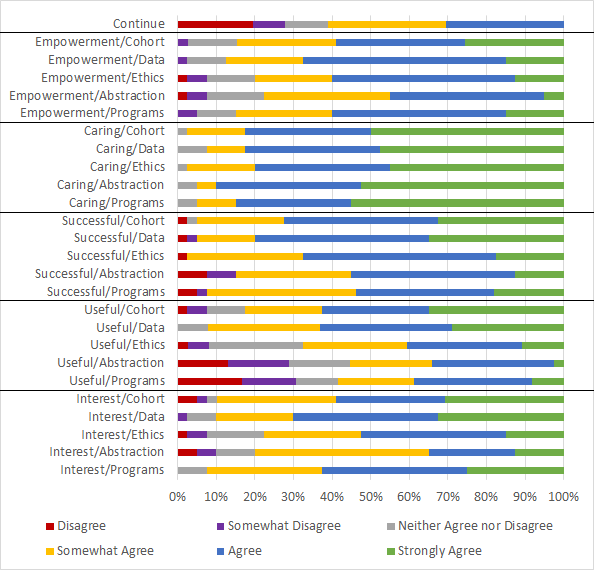
\includegraphics[width=.47\textwidth]{graphics/survey-results}
    \caption{Survey results across motivational and course components}
    \label{fig:survey}
\end{figure}

\begin{figure}[ht!]
\centering
\begin{tabular}{l|lllll}
            & M & U & S & I & C  \\\hline
Abstraction & \textbf{45.8**} & \textbf{69.9**} & \textbf{61.4**} & \textbf{48.8**} & 19.2 \\\hline
Cohort & 9.0 & 11.3 & 3.6 & 7.5 & 7.9 \\\hline
Data & 13.8 & 30.9 & 29.4 & 29.7 & 21.9 \\\hline
Ethics & 30.8 & \textbf{48.5**} & \textbf{41.8**} & \textbf{32.3*} & 18.6 \\\hline
Programs & \textbf{43.7**} & \textbf{82.3**} & \textbf{60.0**} & \textbf{63.8**} & 7.3 \\\hline

%            & C & M & I & S & U  \\\hline
%Abstraction & 15.9 & 26.9      & \textbf{39.1*}  & \textbf{39.4*}    & \textbf{50.1*} \\
%Cohort      & 14.6 & 26.6      & 25.1   & 28.3      & 33.2  \\
%Data        & 11.1 & 16.6       & 19.8    & 25.1     & 30.9  \\
%Ethics      & 17.8 & 24.4      & 21.6   & \textbf{26.5*}    & \textbf{45.3*}  \\
%Programs    & 16.3 & 29.5      & \textbf{27.8*}  & \textbf{38.5*}    & \textbf{71.1*}
\end{tabular}
\caption{Correlation between students' intent to continue vs. components of the course with respect to motivational components (at end of semester)}
\label{tbl-continue}
\end{figure}

Table~\ref{tbl-continue} reveals a potentially important connection between students' motivation with respect to the content and context as compared to their long-term intent to continue in computing.
The vertical categories represent components of the course, while the horizontal categories represent elements of the MUSIC model.
So, for example, the intersection of the row ``Data'' and column ``I'' should be interpreted as ``The correlation between students' interest in learning about real-world data related to their major and their intent to continue learning computing''.
Bolded items are significantly correlated.
Although the correlations are modest, there is a strong connection between students' sense of the usefulness of learning the core course content (and, to a lesser extent, their self-efficacy and interest towards the content) and their intent to continue.
However, there is no significant correlation between students' sense of the usefulness of learning to work with real-world data (the course context) and their intent to continue.
Note that this is despite students expressing more positive responses towards the usefulness of working with real-world data vs. programming.
This makes sense, since students will perceive continuing in Computer Science as being about programming, not about data science.
Our preliminary interpretation of this result is that, if we wish to encourage students to continue learning computing, we should convince them of ways that learning to write programs and learning computing can directly benefit their careers.
Although the small sample size does mitigate the finding, and there are a number of other possible interpretations, it does suggest a worthwhile avenue for future research.

\section{Contribution}

In this paper, we have described a number of innovations that we think will benefit the introductory computing education community.
At its core, the CORGIS project represents a concerted effort to make many excellent datasets available for introductory computing students.
We have introduced a novel architecture to support this process, making it easy to convert an existing dataset into a wide variety of student-ready materials.
Over 40 datasets have already been incorporated into our collection, spanning across disciplines such as education, health, history, and politics.
Not only do we provide beginner programmer-friendly libraries in multiple common introductory languages, we also provide web-based tools for quickly accessing the datasets without programming.
We describe a number of ways these libraries and tools can be used in a course in order to satisfy both conceptual and programming learning objectives.
Finally, we report on survey results of the integration of these datasets into a computational thinking course.
These results reveal not just the success of the integration, but also suggest a potential path for bringing students more solidly into computing.


\section{Conclusions and Future Work}

The RealTimeWeb and CORGIS projects have been developed over the past 4 years.
At this point, it is useful to reflect on the future work needed for the project.

First, further research must be done to evaluate the impact of this type of context on learners' cognition and motivation, similar to the longitudinal studies performed by the Media Computation project~\cite{guzdial2013exploring}.
Second, the quantity, quality, and diversity of datasets needs to continue to grow in order to meet the demand of students entering introductory computing.
Although understanding the impact on learners is relatively straightforward, expanding the project's collection raises a number of technical issues.

A major limitation of dataset preparation is the expertise required to convert datasets into a format suitable for processing.
Although there is significant dedicated research to lowering barriers for this process, it is still the work of a seasoned programmer.
Further, every dataset demands some level of domain knowledge to correctly and meaningfully arrange the fields.
We currently use only open-access, unprotected datasets, thus limiting the field sharply.
One unexplored direction is the creation of artificial datasets based on known characteristics of existing but unsuitable datasets.
For example, a detailed dataset representing hospital records would normally be protected by HIPAA.
But an artificial collection of records might be generated from the real data, suitable for open use.
Although such datasets would not allow students to discover trends and facts about reality, we could use statistical techniques to ensure some relative accuracy of the data.
Further research must be conducted to see if this is technically feasible and still perceived as authentic by students.

We hope that interested readers will try out the materials at \url{https://think.cs.vt.edu/corgis}, and consider submitting their own datasets to expand our collection.

\section{Acknowledgments}

We gratefully acknowledge the support of the National Science Foundation under Grants NSF DGE 0822220, NSF DUE 1444094, and NSF IUSE
1624320.


\bibliographystyle{abbrv}
\bibliography{references}  % sigproc.bib is the name of the Bibliography in this case

\end{document}